\begin{flushright} {\tiny {\color{gray} (tikz\_3x2\_q2.tex)}} \end{flushright}
%~~~~~~~~~~~~~~~~~~~~~~~~~~~~~~~~~~~~~~~~~~~~~~~~~~~~~~~~~~~~~~~~~~~~~~~~~~~~~~~~~~~~~~~~~~~~~~~~~~

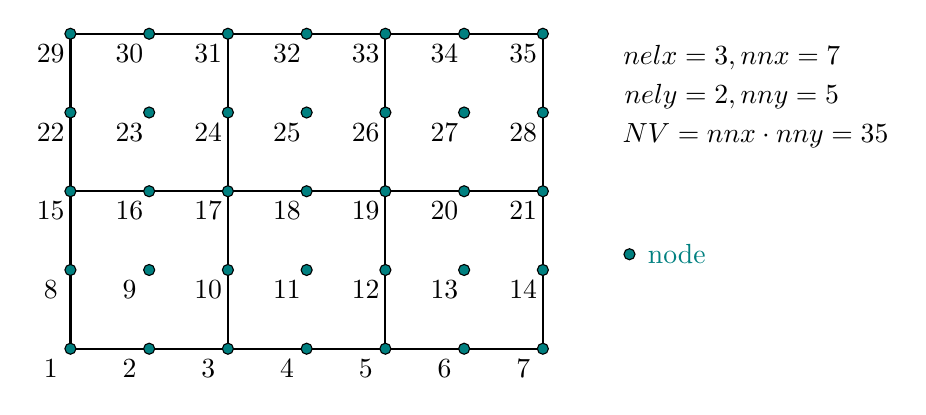
\begin{tikzpicture}
%\draw[step=0.5cm,gray,very thin] (0,0) grid (9,5); %background grid

\draw[thick] (1,1) -- (7,1) -- (7,5) -- (1,5) -- cycle;  
\draw[thick] (1,3) -- (7,3) ;
\draw[thick] (3,1) -- (3,5) ;
\draw[thick] (5,1) -- (5,5) ;

\draw[black,fill=teal] (1,1)     circle (2pt); 
\draw[black,fill=teal] (2,1)     circle (2pt); 
\draw[black,fill=teal] (3,1)     circle (2pt); 
\draw[black,fill=teal] (4,1)     circle (2pt); 
\draw[black,fill=teal] (5,1)     circle (2pt); 
\draw[black,fill=teal] (6,1)     circle (2pt); 
\draw[black,fill=teal] (7,1)     circle (2pt); 

\draw[black,fill=teal] (1,2)     circle (2pt); 
\draw[black,fill=teal] (2,2)     circle (2pt); 
\draw[black,fill=teal] (3,2)     circle (2pt); 
\draw[black,fill=teal] (4,2)     circle (2pt); 
\draw[black,fill=teal] (5,2)     circle (2pt); 
\draw[black,fill=teal] (6,2)     circle (2pt); 
\draw[black,fill=teal] (7,2)     circle (2pt); 

\draw[black,fill=teal] (1,3)     circle (2pt); 
\draw[black,fill=teal] (2,3)     circle (2pt); 
\draw[black,fill=teal] (3,3)     circle (2pt); 
\draw[black,fill=teal] (4,3)     circle (2pt); 
\draw[black,fill=teal] (5,3)     circle (2pt); 
\draw[black,fill=teal] (6,3)     circle (2pt); 
\draw[black,fill=teal] (7,3)     circle (2pt); 

\draw[black,fill=teal] (1,4)     circle (2pt); 
\draw[black,fill=teal] (2,4)     circle (2pt); 
\draw[black,fill=teal] (3,4)     circle (2pt); 
\draw[black,fill=teal] (4,4)     circle (2pt); 
\draw[black,fill=teal] (5,4)     circle (2pt); 
\draw[black,fill=teal] (6,4)     circle (2pt); 
\draw[black,fill=teal] (7,4)     circle (2pt); 

\draw[black,fill=teal] (1,5)     circle (2pt); 
\draw[black,fill=teal] (2,5)     circle (2pt); 
\draw[black,fill=teal] (3,5)     circle (2pt); 
\draw[black,fill=teal] (4,5)     circle (2pt); 
\draw[black,fill=teal] (5,5)     circle (2pt); 
\draw[black,fill=teal] (6,5)     circle (2pt); 
\draw[black,fill=teal] (7,5)     circle (2pt); 

\node[] at (0.75,0.75) {1};
\node[] at (1.75,0.75) {2};
\node[] at (2.75,0.75) {3};
\node[] at (3.75,0.75) {4};
\node[] at (4.75,0.75) {5};
\node[] at (5.75,0.75) {6};
\node[] at (6.75,0.75) {7};

\node[] at (0.75,1.75) {8};
\node[] at (1.75,1.75) {9};
\node[] at (2.75,1.75) {10};
\node[] at (3.75,1.75) {11};
\node[] at (4.75,1.75) {12};
\node[] at (5.75,1.75) {13};
\node[] at (6.75,1.75) {14};

\node[] at (0.75,2.75) {15};
\node[] at (1.75,2.75) {16};
\node[] at (2.75,2.75) {17};
\node[] at (3.75,2.75) {18};
\node[] at (4.75,2.75) {19};
\node[] at (5.75,2.75) {20};
\node[] at (6.75,2.75) {21};

\node[] at (0.75,3.75) {22};
\node[] at (1.75,3.75) {23};
\node[] at (2.75,3.75) {24};
\node[] at (3.75,3.75) {25};
\node[] at (4.75,3.75) {26};
\node[] at (5.75,3.75) {27};
\node[] at (6.75,3.75) {28};

\node[] at (0.75,4.75) {29};
\node[] at (1.75,4.75) {30};
\node[] at (2.75,4.75) {31};
\node[] at (3.75,4.75) {32};
\node[] at (4.75,4.75) {33};
\node[] at (5.75,4.75) {34};
\node[] at (6.75,4.75) {35};

\draw[black,fill=teal] (8.1,2.2) circle (2pt); 
\node[] at (8.7,2.2) {{\color{teal}node}};

\node[] at (9.4,4.7) {$nelx=3, nnx=7$};
\node[] at (9.4,4.2) {$nely=2, nny=5$};
\node[] at (9.7,3.7) {$NV=nnx\cdot nny=35$};

\end{tikzpicture}
